\documentclass[graybox]{svmult}

\usepackage[bottom]{footmisc}
\usepackage[utf8]{inputenc}
\usepackage{graphicx}
\usepackage{listings}
\usepackage{makeidx}
\usepackage{multicol}
\usepackage{newtxtext}
\usepackage{newtxmath}
\usepackage{url}
\RequirePackage[l2tabu, orthodox]{nag}

% Allow PDF 1.7 documents to be included with \includegraphics
\pdfminorversion=7

\graphicspath{{./img/}}

% listing
\lstset{%
  language={C},
  basicstyle={\small\ttfamily},%
  identifierstyle={\small\ttfamily},%
  commentstyle={\small\itshape},%
  keywordstyle={\small\bfseries},%
  ndkeywordstyle={\small\ttfamily},%
  stringstyle={\small\ttfamily},%
  frame={tb},%
  breaklines=true,%
  columns=[l]{fullflexible},%
  numbers=left,%
  numberstyle={\scriptsize},%
  stepnumber=1,%
  numbersep=1em,%
  lineskip=-0.5ex,%
  mathescape,%
  xleftmargin=2em,%
  framexleftmargin=1.5em,%
}

\makeindex

\begin{document}

\title*{An MPI Framework for HPC Clusters Deployed with Software-Defined
Networking}
% Use \titlerunning{Short Title} for an abbreviated version of
% your contribution title if the original one is too long
\author{Keichi Takahashi, Susumu Date, Yasuhiro Watashiba, Yoshiyuki Kido,
Shinji Shimojo}
% Use \authorrunning{Short Title} for an abbreviated version of
% your contribution title if the original one is too long
\institute{Keichi Takahashi \at Nara Institute of Science and Technology,
8916-5 Takayama, Ikoma, Nara, Japan\\ \email{keichi@is.naist.jp}
\and Susumu Date, Yasuhiro Watashiba, Yoshiyuki Kido, Shinji Shimojo \at
Cybermedia Center, Osaka University, 5-1 Mihogaoka, Ibaraki, Osaka, Japan\\
\email{{date, watashiba-y, kido, shimojo}@cmc.osaka-u.ac.jp}}
%
% Use the package "url.sty" to avoid
% problems with special characters
% used in your e-mail or web address
%
\maketitle

\abstract*{Each chapter should be preceded by an abstract (no more than 200
words) that summarizes the content. The abstract will appear \textit{online}
at \url{www.SpringerLink.com} and be available with unrestricted access. This
allows unregistered users to read the abstract as a teaser for the complete
chapter. Please use the 'starred' version of the \texttt{abstract} command for
typesetting the text of the online abstracts (cf. source file of this chapter
template \texttt{abstract}) and include them with the source files of your
manuscript. Use the plain \texttt{abstract} command if the abstract is also to
appear in the printed version of the book.}

\abstract{Each chapter should be preceded by an abstract (no more than 200
words) that summarizes the content. The abstract will appear \textit{online}
at \url{www.SpringerLink.com} and be available with unrestricted access. This
allows unregistered users to read the abstract as a teaser for the complete
chapter.\newline\indent Please use the 'starred' version of the
\texttt{abstract} command for typesetting the text of the online abstracts
(cf. source file of this chapter template \texttt{abstract}) and include them
with the source files of your manuscript. Use the plain \texttt{abstract}
command if the abstract is also to appear in the printed version of the book.}

\section{Introduction}

Lorem Ipsum is simply dummy text of the printing and typesetting industry.
Lorem Ipsum has been the industry's standard dummy text ever since the 1500s,
when an unknown printer took a galley of type and scrambled it to make a type
specimen book. It has survived not only five centuries, but also the leap into
electronic typesetting, remaining essentially unchanged. It was popularised in
the 1960s with the release of Letraset sheets containing Lorem Ipsum passages,
and more recently with desktop publishing software like Aldus PageMaker
including versions of Lorem Ipsum~\cite{Takahashi2014}. including versions of
Lorem Ipsum~\cite{Takahashi2015}. including versions of Lorem
Ipsum~\cite{Takahashi2017}. including versions of Lorem
Ipsum~\cite{Takahashi2018}. including versions of Lorem
Ipsum~\cite{Dashdavaa2014}.


\section{Background}

\subsection{SDN-enhanced MPI}

MPI~\cite{MPIForum2012}

\subsection{Job Scheduler}

A job scheduler is a system that accepts \textit{job} submissions from users and
dispatch the

Examples of job schedulers used in production HPC systems include
Slurm~\cite{Yoo2003}, PBS
Professional\footnote{\url{https://www.pbspro.org/}},
Torque\footnote{\url{https://www.adaptivecomputing.com/products/torque/}} and
UNIVA Grid Engine\footnote{\url{http://www.univa.com/products/}}. In this
paper, Slurm is assumed as it is one of the most widely adopted open-source
job schedulers.

Figure~\ref{kt:fig:slurm} shows the architecture of Slurm. Slurm employs a
master-worker architecture like many other job schedulers. The master accepts
job requests from users and

Here, it is assumed
that the cluster has three types of node: login node, head node and compute
node.

Like many job
schedulers, Slurm employs a master-worker architecture, where the master
accepts from

\begin{figure}
    \centering
    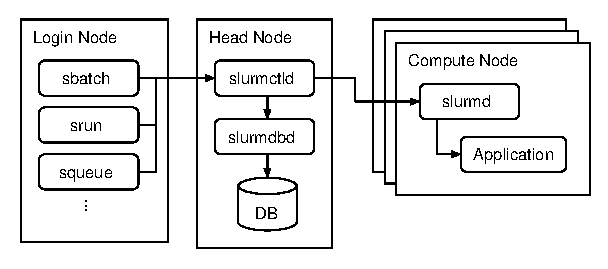
\includegraphics{slurm}
    \caption{Architecture of Slurm}%
    \label{kt:fig:slurm}
\end{figure}

\subsection{Challenges and Goal}

\section{Proposal}

\subsection{Overview}

Figure~\ref{kt:fig:architecture} shows the overall architecture of the
proposed SDN-enhanced MPI framework.

The scheduler plugin and the interconnect manager use
gRPC\footnote{\url{https://grpc.io/}} to communicate with one another. We have
chosen gRPC, which is an RPC framework built on top of HTTP/2, because it
can automatically generate server and client based on the interface
definition.

\begin{figure}
    \centering
    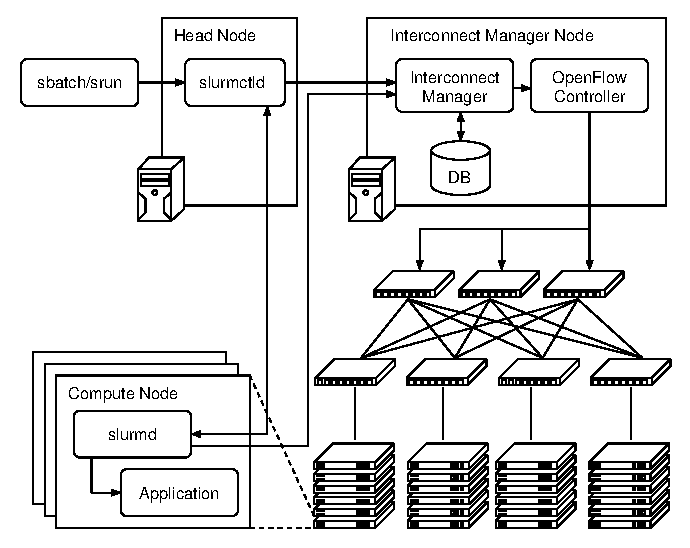
\includegraphics{architecture}
    \caption{Overall architecture}%
    \label{kt:fig:architecture}
\end{figure}

\subsection{Interconnect Manager}

The interconnect manager is responsible for computing and installing optimal
routes for each job.

\begin{itemize}
    \item Receiving notifications from srun and slurmd
    \item Persisting the state of jobs to a database
    \item Computing routes
    \item Installing routes to interconnect by talking to the OpenFlow
        controller.
\end{itemize}


The builtin REST API server of Ryu.

Ryu\footnote{\url{https://osrg.github.io/ryu/}}

OpenFlow~\cite{McKeown2008}
SQLite\footnote{\url{https://www.sqlite.org/index.html}}

\subsection{Scheduler Plugin}

The scheduler plugin is responsible for

-

Slurm provides a plugin mechanism called Slurm Plug-in Architecture for Node
and job Control (SPANK). SPANK

Furthermore,

This plugin is inserted into srun and slurmd

srun: Sends job ID, name, uid/gid of user, number of tasks and communication
pattern name to the interconnect manager when a job is submitted.
slurmd: Sends job id, MPI rank, node ID and node name to interconnect manager
when a process consisting a job starts or exits. Blocks until the routings
have been setup in the interconnect.

\begin{lstlisting}
#!/bin/bash
#
#SBATCH --job-name=test_omp
#SBATCH --output=res_omp.txt
#
#SBATCH --ntasks=1
#SBATCH --cpus-per-task=4
#SBATCH --time=10:00
#SBATCH --mem-per-cpu=100
#SBATCH --comm-pattern=cg-c-128
\end{lstlisting}


\section{Evaluation}

\subsection{Evaluation Environment}

\begin{figure}
    \centering
    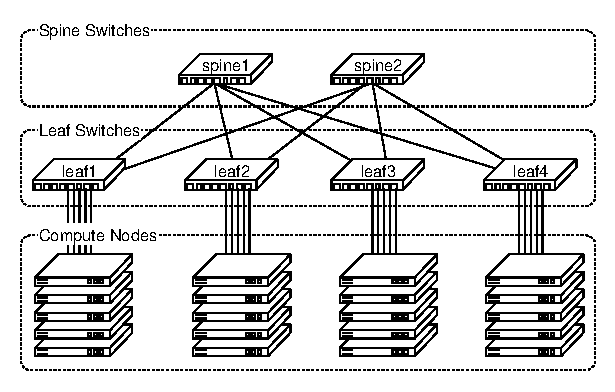
\includegraphics{evaluation_cluster}
    \caption{Cluster used for evaluation}%
    \label{kt:fig:cluster}
\end{figure}

\subsection{Evaluation Result}

\begin{figure}
    \centering
    \includegraphics{benchmark_result}
    \caption{Benchmark results using miniapps}%
    \label{kt:fig:benchmark}
\end{figure}

\section{Conclusion}

\bibliographystyle{spmpsci}
\bibliography{references}

\end{document}
